\documentclass[a4paper,12pt]{article}

%%% Работа с русским языком % для pdfLatex
\usepackage{cmap}					% поиск в~PDF
\usepackage{mathtext} 				% русские буквы в~фомулах
\usepackage[T2A]{fontenc}			% кодировка
\usepackage[utf8]{inputenc}			% кодировка исходного текста
\usepackage[english,russian]{babel}	% локализация и переносы
\usepackage{indentfirst} 			% отступ 1 абзаца

%%% Работа с русским языком % для XeLatex
%\usepackage[english,russian]{babel}   %% загружает пакет многоязыковой вёрстки
%\usepackage{fontspec}      %% подготавливает загрузку шрифтов Open Type, True Type и др.
%\defaultfontfeatures{Ligatures={TeX},Renderer=Basic}  %% свойства шрифтов по умолчанию
%\setmainfont[Ligatures={TeX,Historic}]{Times New Roman} %% задаёт основной шрифт документа
%\setsansfont{Comic Sans MS}                    %% задаёт шрифт без засечек
%\setmonofont{Courier New}
%\usepackage{indentfirst}
%\frenchspacing

%%% Дополнительная работа с математикой
\usepackage{amsfonts,amssymb,amsthm,mathtools}
\usepackage{amsmath}
\usepackage{icomma} % "Умная" запятая: $0,2$ --- число, $0, 2$ --- перечисление
\usepackage{upgreek}

%% Номера формул
%\mathtoolsset{showonlyrefs=true} % Показывать номера только у тех формул, на которые есть \eqref{} в~тексте.

%%% Страница
\usepackage{extsizes} % Возможность сделать 14-й шрифт

%% Шрифты
\usepackage{euscript}	 % Шрифт Евклид
\usepackage{mathrsfs} % Красивый матшрифт

%% Свои команды
\DeclareMathOperator{\sgn}{\mathop{sgn}} % создание новой конанды \sgn (типо как \sin)
\usepackage{csquotes} % ещё одна штука для цитат
\newcommand{\pd}[2]{\ensuremath{\cfrac{\partial #1}{\partial #2}}} % частная производная
\newcommand{\abs}[1]{\ensuremath{\left|#1\right|}} % модуль
\renewcommand{\phi}{\ensuremath{\varphi}} % греческая фи
\newcommand{\pogk}[1]{\!\left(\cfrac{\sigma_{#1}}{#1}\right)^{\!\!\!2}\!} % для погрешностей

% Ссылки
\usepackage{color} % подключить пакет color
% выбрать цвета
\definecolor{BlueGreen}{RGB}{49,152,255}
\definecolor{Violet}{RGB}{120,80,120}
% назначить цвета при подключении hyperref
\usepackage[unicode, colorlinks, urlcolor=blue, linkcolor=blue, pagecolor=blue, citecolor=blue]{hyperref} %синие ссылки
%\usepackage[unicode, colorlinks, urlcolor=black, linkcolor=black, pagecolor=black, citecolor=black]{hyperref} % для печати (отключить верхний!)


%% Перенос знаков в~формулах (по Львовскому)
\newcommand*{\hm}[1]{#1\nobreak\discretionary{}
	{\hbox{$\mathsurround=0pt #1$}}{}}

%%% Работа с картинками
\usepackage{graphicx}  % Для вставки рисунков
\graphicspath{{images/}{images2/}}  % папки с картинками
\setlength\fboxsep{3pt} % Отступ рамки \fbox{} от рисунка
\setlength\fboxrule{1pt} % Толщина линий рамки \fbox{}
\usepackage{wrapfig} % Обтекание рисунков и таблиц текстом
\usepackage{multicol}

%%% Работа с таблицами
\usepackage{array,tabularx,tabulary,booktabs} % Дополнительная работа с таблицами
\usepackage{longtable}  % Длинные таблицы
\usepackage{multirow} % Слияние строк в~таблице
\usepackage{caption}
\captionsetup{labelsep=period, labelfont=bf}

%%% Оформление
\usepackage{indentfirst} % Красная строка
%\setlength{\parskip}{0.3cm} % отступы между абзацами
%%% Название разделов
\usepackage{titlesec}
\titlelabel{\thetitle.\quad}
\renewcommand{\figurename}{\textbf{Рис.}}		%Чтобы вместо figure под рисунками писал "рис"
\renewcommand{\tablename}{\textbf{Таблица}}		%Чтобы вместо table над таблицами писал Таблица

%%% Теоремы
\theoremstyle{plain} % Это стиль по умолчанию, его можно не переопределять.
\newtheorem{theorem}{Теорема}[section]
\newtheorem{proposition}[theorem]{Утверждение}

\theoremstyle{definition} % "Определение"
\newtheorem{definition}{Определение}[section]
\newtheorem{corollary}{Следствие}[theorem]
\newtheorem{problem}{Задача}[section]

\theoremstyle{remark} % "Примечание"
\newtheorem*{nonum}{Решение}
\newtheorem{zamech}{Замечание}[theorem]

%%% Правильные мат. символы для русского языка
\renewcommand{\epsilon}{\ensuremath{\varepsilon}}
\renewcommand{\phi}{\ensuremath{\varphi}}
\renewcommand{\kappa}{\ensuremath{\varkappa}}
\renewcommand{\le}{\ensuremath{\leqslant}}
\renewcommand{\leq}{\ensuremath{\leqslant}}
\renewcommand{\ge}{\ensuremath{\geqslant}}
\renewcommand{\geq}{\ensuremath{\geqslant}}
\renewcommand{\emptyset}{\varnothing}

%%% Для лекций по инфе
\usepackage{alltt}
\newcounter{infa}[section]
\newcounter{num}
\definecolor{infa}{rgb}{0, 0.2, 0.89}
\definecolor{infa1}{rgb}{0, 0.3, 1}
\definecolor{grey}{rgb}{0.5, 0.5, 0.5}
\newcommand{\tab}{\ \ \ }
\newcommand{\com}[1]{{\color{grey}\##1}}
\newcommand{\num}{\addtocounter{num}{1}\arabic{num}\tab}
\newcommand{\defi}{{\color{infa}def}}
\newcommand{\globali}{{\color{infa}global}}
\newcommand{\ini}{{\color{infa}in}}
\newcommand{\rangei}{{\color{infa}range}}
\newcommand{\fori}{{\color{infa}for}}
\newcommand{\ifi}{{\color{infa}if}}
\newcommand{\elsei}{{\color{infa}else}}
\newcommand{\printi}{{\color{infa1}print}}
\newcommand{\enumeratei}{{\color{infa1}enumerate}}
\newcommand{\maxi}{{\color{infa}max}}
\newcommand{\classi}{{\color{infa}class}}
\newcommand{\returni}{{\color{infa}return}}
\newcommand{\elifi}{{\color{infa}elif}}
\newenvironment{infa}[1]{
	
	\vspace{0.5cm}
	\addtocounter{infa}{1}%
	\noindent{\large \textbf{Программа №\thesection.\arabic{infa}.}\ \textbf{#1}}%
	\begin{alltt}%
	}{\end{alltt}
	\setcounter{num}{0}
	\vspace{0.1cm}}
%Пример кода:
%\begin{infa}{Поразрядная сортировка}
%	\ \num \defi count_sort(a):\tab \com{определяет нашу функцию}
%	\ \num \tab m = \maxi(a)+1
%	\ \num \tab q = [0]*m
%	\ \num \tab \fori x \ini a:
%	\ \num \tab \tab q[x] += 1
%	\ \num \tab pos = 0
%	\ \num \tab \fori x \ini q:
%	\ \num \tab \tab \fori i \ini \rangei(q[x]):
%	\ \num \tab \tab \tab a[pos] = x
%	\num \tab \tab \tab pos += 1
%\end{infa}

\usepackage[left=1.27cm,right=1.27cm,top=1.27cm,bottom=2cm]{geometry}
%\hbox to\textwidth{команда колонтитула}
\begin{document}
\newcounter{lec}
\newcommand{\lec}[1]{\addtocounter{lec}{1} \setcounter{section}{0}%
\begin{center}
{\LARGE ЛЕКЦИЯ \arabic{lec}%
\vspace{2mm}%

\textbf{#1}%
}
\end{center}
}
\newpage
\
\setcounter{lec}{16}
\lec{Графы}
\section{Графы}
Граф --- множество вершин и инцедентных им ребер.
$$G=(V, E)$$
$$v \in V, \qquad e \in E $$
Говорят, что ребро $e$ инцедентно вершине $v$, если она является его концом.

Допустимы графы:
$$G = (\varnothing, \varnothing)$$
$$G = ({1}, \varnothing)$$
Недопустим граф:
$$G = (\varnothing, {a})$$

Граф --- "упрощенная модель".

У ребра \underline{2 конца}. Это не обязательно отрезок. 

Ребро может быть петлей.

2 разных ребра могут быть инцедентно двум вершинам --- кратные ребра.

У классического графа 2 конца. Но может быть ориентированный граф. Т.е. либо у ребра 2 конца, либо у него есть начало и конец. Тогда ребро называется дуга. Короткое название \textbf{орграф}.

\section{Задача Эйлера о семи кёнигсбергских мостах}
Как пройти по всем городским мостам (через реку Преголя), не проходя ни по одному из них дважды?
\begin{figure}[h!]
	\noindent\centering{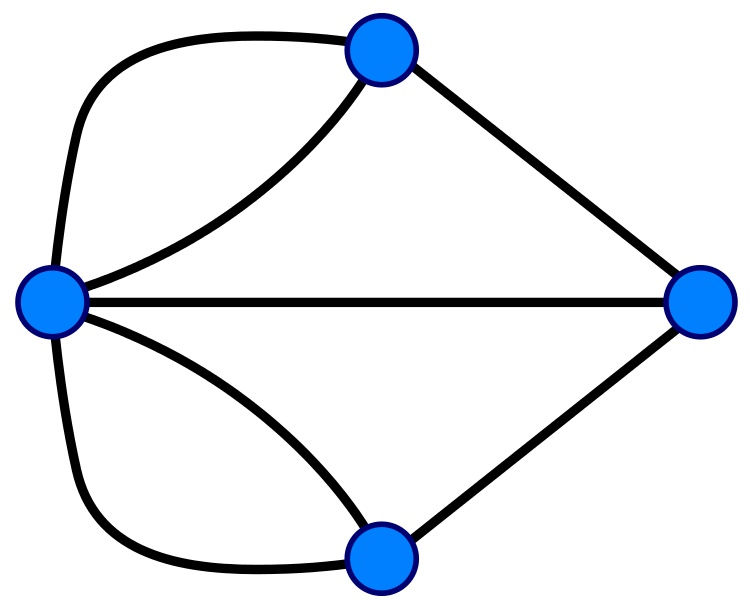
\includegraphics[width=8cm]{graph.jpg}}
	\caption{Граф к задаче о мостах}
	\label{fp_2}
	\vspace{-0.5cm}
\end{figure}

\textit{Введем дополнительные понятия:}

Степень вершины --- количество инцедентных ей ребер.

Граф G' = (V', E') является подграфом G, если V' $\subset$ V, E' $\subset$ E.

Путь --- последовательность ребер (в которой конец каждого ребра есть начало следующего).

Путь тоже является графом, а точнее это орграф, подграф исходного.

Любой неориентированный граф можно представить как ориентированный.

Цикл --- путь, в котором начало пути (начало первого ребра) совпадает с концом (конец последнего ребра).

Рассмотрим граф A---B.

Возможны пути
$$[AB, BA]$$

Простой путь --- путь, у которого не повторяются ребра (вершины повторятся могут).

Простой цикл ---  цикл, у которого не повторяются ребра (вершины повторятся могут).

\textbf{Вернемся к задаче.}

Пусть вершина верхняя вершина --- старт. Пройдем по ребру и выкинем его (т.е. степень у вершины понизится). Продолжим процесс аналогично. В итоге какой бы путь мы не строили, степени у всех промежуточных вершин понизятся на четное число, а у вершин финиша и начала понизятся на нечетное число. Т.о. это невозможно. Подробнее \href{https://ru.wikipedia.org/wiki/%D0%97%D0%B0%D0%B4%D0%B0%D1%87%D0%B0_%D0%BE_%D1%81%D0%B5%D0%BC%D0%B8_%D0%BA%D1%91%D0%BD%D0%B8%D0%B3%D1%81%D0%B1%D0%B5%D1%80%D0%B3%D1%81%D0%BA%D0%B8%D1%85_%D0%BC%D0%BE%D1%81%D1%82%D0%B0%D1%85}{в вики}.

Эйлеров цикл --- простой цикл, включающий все ребра графа.

Эйлеров граф --- граф, в котором существует Эйлеров цикл.

Полуйэлеров граф --- граф, в котором есть Эйлеров путь, но нет Эйлерого цикла.

\section{Связность графов}
Граф является связным, если для $\forall A,B \in V$ существует путь от $A$ к $B$.\\
$A\longrightarrow B\longrightarrow C$ --- несвязный граф.

Компонент связности --- связный подграф, в который включены все вершины исходного, связаные с принадлежащими подграфами. Связный граф имеет 1 компоненту связности. Крайний случай: вершины без ребер. Количество компонент связности от 1 до количества вершин.

Слабая связность --- "забываем"\  про направленность графов и смотрим на связность.

Сильно связный граф --- граф связан при условии направленности.

"Вес"\  ребра --- некоторая числовая характеристика ребра (расстояние, время прохождения, стоимость, энергия реакции и т.д.). Это необязательно положительное число.

Взвешенный граф --- граф, у которого все ребра имеют вес.

\section{Хранение графа в памяти ПК}
Введем понятие: смежные вершины --- <<соседи>>, т.е. это вершины, которые имеют общее ребро. Ациклический граф --- орграф без цикла.

\subsection{Формы хранения}
Есть 3 основные формы хранения:\\
1. Список ребер (множество ребер)
\begin{center}
AB 5\\
BC 3\\
CD 1\\
DE 2\\
\end{center}
2. Матрица смежности\\
Матрица смежности не умеет хранить кратные ребра (если только массив не трехмерный (но это бред)).

\begin{center}
\begin{tabular}{|c|c|c|c|c|c|}
	\hline 
	& A & B & C & D & E \\ 
	\hline 
	A & x & 1 & 0 & 0 & 0 \\ 
	\hline 
	B & 1 & x & 1 & 0 & 0 \\ 
	\hline 
	C & 0 & 1 & x & 1 & 0 \\ 
	\hline 
	D & 0 & 0 & 1 & x & 1 \\ 
	\hline 
	E & 0 & 0 & 0 & 1 & x \\ 
	\hline 
\end{tabular}
\end{center}

Можно  также составить матрицу взвешенности, если записать в эту матрицу вес каждого ребра.

\noindent3. Списки смежности\\
\begin{align*}
&A : B\\
&B : A, \quad C\\
&C : B, \quad D\\
&D : C, \quad E\\
&E : D\\
\end{align*}

\subsection{Реализация на Python}
\begin{enumerate}
	\item Список ребер
\begin{infa}{}
\num G = ('AB', 5),
\num \tab ('BC', 3),
\num \tab ('CD', 1),
\num \tab ('DE', 2)
\end{infa}
Но кортежами не очень удобно.
\begin{infa}{}
\num G = {'AB' : 5
\num \tab 'BC' : 3
\num \tab 'CD' : 1
\num \tab 'DE': 2}
\end{infa}

Задачи:
\begin{enumerate}
\item Проверка смежности.
\item Перебор "соседей".
\end{enumerate}

\item Таблица смежности
\begin{infa}{}
\num G = [[0,1,0,0,0],
\num \tab [1,0,1,0,0],
\num \tab [0,1,0,1,0],
\num \tab [0,0,1,0,1],
\num \tab [0,0,0,1,0]]
\end{infa}
Решение задач:
\begin{enumerate}
\item Проверка смежностей
\begin{infa}{}
G[i][k] == 1\text{ - значит смежные}
\end{infa}

\item Перебор соседей: нужно пробежать по строке.
\end{enumerate}

\item Списки смежности

Словарь множеств смежностей:
\begin{infa}{}
\num G = \{'A':\{'B':5\}
\num \tab 'B':\{'A':5, 'C':3\}
\num \tab 'C': \{'B':3, 'D':1\}
\num \tab 'D': \{'C':1, 'E':2\}
\num \tab 'E': \{'D':2\}\}
\end{infa}
Проверка факта смежностей:
\begin{alltt}
	'B' in G['A'] \com{O(1)}
\end{alltt}

Перебор соседей:
\begin{alltt}
for v in G['A']:
\end{alltt}
$O(N_{e_{max}})$, $N_e$ - средняя степень вершины.

\end{enumerate}

\begin{center}
	\vfill \emph{{\small Г. С. Демьянов, \href{https://vk.com/id37346992}{ВК}}}
\end{center}






\end{document} 